\chapter{Metodología}
\label{metodologia}

\section{Metodología}
La metodología llevada a cabo durante el proyecto es una creación propia basada en caraterísticas
copiadas de metodologías ágiles como el \textbf{'Scrum'} y adaptadas a la forma de trabajar propia.
La idea es estructurar todo el proyecto en diversas iteraciones y durante estas marcarse
objetivos y/o tareas con el fin de añadir funcionalidades completas.

El uso de \textbf{iteraciones} para dividir la carga de trabajo y agrupar tareas nos ayudará
a conseguir acotar la duración de algunas tareas y marcarnos objetivos a corto/medio
plazo. Además de separar por funciones el proyecto, las tareas que conllevan su desarrollo
también deberemos analizarlas e intentar reducir su tamaño y carga lo máximo posible, esto
permite obtener una sensación de éxito de forma rápida lo cual ayuda a mantener una moral y 
motivación altas.

Para poner un ejemplo de como elaborar esta separación por subtareas, el objetivo que vamos a
usar es ``dibujar elementos por pantalla''. Como estamos en un proyecto básado en \ac{ECS} rápidamente
vemos que vamos a requerir mínimo un componente de dibujado \textit{(RenderCmp)} y un 
``RenderSystem'' el cual se encargará de recoger todos los elementos visuales y hacer las
llamadas necesarias para dibujarlos. \\
En caso de no tener una librería de dibujado, otra tarea podría ser el buscar una que sea capaz
de realizar el trabajo requerio y/o implementar una propia
\footnote{Esto supondría una serie de tareas en base a la cantidad de funcionalidades que se requieran.}. 

Para ayudar a la planificación del trabajo usaremos la herramienta `Trello'
\footnote{Página de `Trello': \url{https://trello.com/es}}
la cual nos permitirá crear diversas listas según el ámbito o el estado de
desarrollo de las distintas tareas que contendrán, cada tarea se ve representada con
una tarjeta la cual puede tener una serie de subtareas asociadas dentro. Esto nos
permitirá tener un registro de todas las labores que quedan por hacer en cada iteración y
cuales ya estan termiandas completamente, además podremos conservar las listas de las tareas
realizadas en iteraciones anteriores para futuras revisiones.

Otra herramienta de control que usaremos durante el desarrollo será `Toggl'
\footnote{Página de `Toggl':  \url{https://toggl.com}}
la cual nos permitirá llevar a cabo un registro de las horas que dedicamos en cada tarea
y agrupar tareas en función del campo de estudio o parte del desarrollor al que pertecen.

\begin{figure}[ht]
\centering

\includegraphics[width=0.35\textwidth]{imagenes/metodologia/logo-trello.png}
\caption{Logo de Trello}
\label{img:trello}
\end{figure}

\begin{figure}[htb]
\centering

\includegraphics[width=0.35\textwidth]{imagenes/metodologia/logo-toggl.png}
\caption{Logo de Toggl}
\label{img:toggl}
\end{figure}

\section{Estructura de una iteración}
Con el fin de trabajar de la mejor forma posible, a lo largo de cada iteración encontramos una 
serie de fases/tareas organizativas que guian el flujo de trabajo.    

\begin{figure}[hbt]
\centering
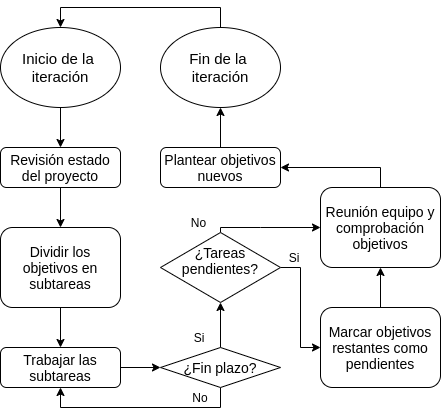
\includegraphics[width=0.48\textwidth]{imagenes/metodologia/Flow-iteracion.png}
\caption{Diagrama de iteración}
\label{img:fases_it}
\end{figure}

El inicio de la iteración trae consigo un análisis y revisado del proyecto, que lo último
implementado esté en un estado aceptable y todo preparado para recibir las futuras adiciones
al proyecto si es que las va a haber.

Una vez esté todo correcto procedemos al estudio y división de las futuras tareas, a la vez 
que las categorizamos según la temática o aspecto del proyecto que se trabaje. \\
Con una visión global de todo el trabajo podemos organizar como vamos a
abordar el desarrollo, analizar si tenemos dependencias entre tareas y acto seguido empezar. \\
Por lo general suelen surgir inconvenientes o nuevas necesidades durante las iteraciones las
cuales nos harán rehacer, posponer o simplemente añadir algunas tareas, por lo que es posible
tener que ampliar de forma puntual este apartado a lo largo de la iteración.

Cuando el apartado organizativo esté terminado (sin tener en cuenta contratiempos) lo único 
que queda por hacer es entrar de lleno en el desarrollo, esta fase se extenderá hasta que
se termine el plazo de la iteración o se acaben los objetivos propuestos. 

Conforme se acerca el final de la iteración, lo último es una reunión de control donde 
se comprueba el porcentaje del trabajo propuesto que ha sido completado, posibles problemas 
encontrados durante la iteración y que soluciones se han aportado (en el caso de haber 
encontrado una). Una vez la discusión termina se procede a marcar las nuevos objetivos
, terminando así la actual iteración y comenzando la siguiente en caso de no finalizar 
todavía el desarrollo del proyecto.







